%%%%%%%%%%%%%%%%%%%%%%%%%%%%%%%%%%%%%%%%%%%%%%%%%%%%%%%%%%%%%%%%%%%%%%%%
% Escuela Politécnica Superior de la Universidad de Alicante
% Realizado por: Jose Manuel Requena Plens
% Contacto: info@jmrplens.com / Telegram:@jmrplens
%%%%%%%%%%%%%%%%%%%%%%%%%%%%%%%%%%%%%%%%%%%%%%%%%%%%%%%%%%%%%%%%%%%%%%%%

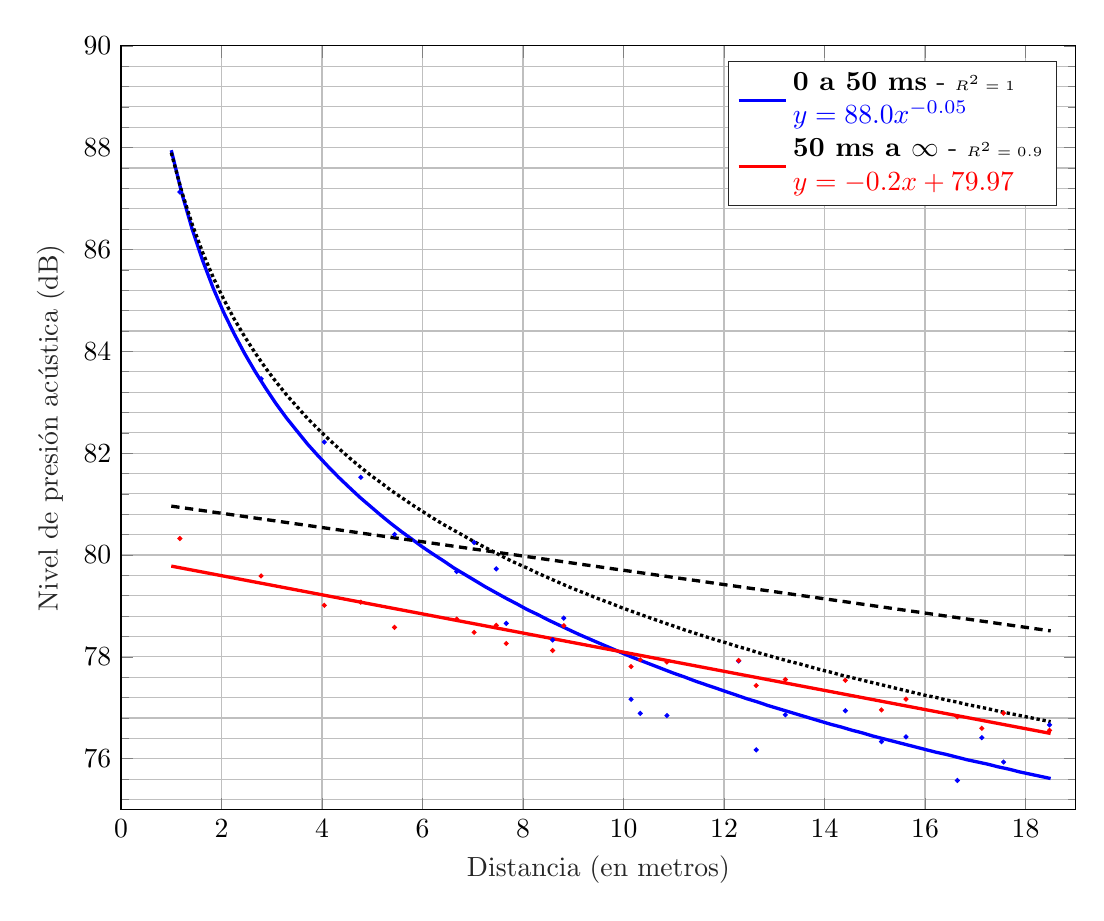
\begin{tikzpicture}

\begin{axis}[%
width=\textwidth,
height=0.8\textwidth,
at={(0\textwidth,0\textwidth)},
scale only axis,
xmin=0,
xmax=19,
xlabel style={font=\color{white!15!black}},
xlabel={Distancia (en metros)},
ymin=75,
ymax=90,
ylabel style={font=\color{white!15!black}},
ylabel={Nivel de presión acústica (dB)},
axis background/.style={fill=white},
xmajorgrids,
xminorgrids,
ymajorgrids,
yminorgrids,
minor y tick num= 4,
legend style={legend cell align=left, align=left, draw=white!15!black}
]
% Curvas EASE
\addplot[color=blue,domain=1:18.5, samples=85,line width=1.2]{87.95*x^(-0.05187)};
\addlegendentry{\textbf{0 a 50 ms} - \tiny{$R^2 = 1$}\\$\color{blue}y = 88.0·x^{-0.05}$}

\addplot[color=red,domain=1:18.5, samples=85,line width=1.2]{-0.1878*x+79.97};
\addlegendentry{\textbf{50 ms a $\infty$} - \tiny{$R^2 = 0.9$}\\$\color{red}y = -0.2·x+79.97$}

% Errores
%\addplot[color=blue, only marks,,mark size=0.7pt,mark=o,error bars/.cd,y dir=both, y explicit] 
%		table [x=x,y=y, y error plus=ymas, y error minus=ymenos]
%			{archivos/graficastikz/UtilErrores.dat};
			
%\addplot[color=red, only marks,mark=o,error bars/.cd,y dir=both, y explicit] 
%		table [x=x,y=y, y error plus=ymas, y error minus=ymenos]
%			{archivos/graficastikz/PerjudicialErrores.dat};


% Curvas insitu
\addplot[color=black,densely dotted,line width=1.2pt,domain=1:18.5, samples=85]{82.4*x^(-0.05)+5.5};
\addplot[color=black,densely dashed,line width=1.2pt,domain=1:18.5, samples=85]{-0.14*x+75.6+5.5};


% Puntos
\addplot [color=blue, only marks,mark size=0.7pt]
  table[row sep=crcr]{%
1.17046999107196	87.1277550611968\\
2.78747197295327	83.4623086675921\\
4.04598566482878	82.2179401358662\\
4.77179211617606	81.5257517559293\\
5.44357419348722	80.4045039689526\\
6.68075594525051	79.6754872626557\\
7.02637886823647	80.2469029713596\\
7.46793144049944	79.7283523968088\\
7.66615940350838	78.6559229050811\\
8.58894638474359	78.3326673816969\\
8.81093071133805	78.7617201801592\\
10.1498768465435	77.1663192028700\\
10.3329569823938	76.8891694043067\\
10.8637010268140	76.8468643393087\\
12.2890194889584	77.9181962233661\\
12.6400158227749	76.1735762643118\\
13.2200605142337	76.8612684404271\\
14.4142290810157	76.9428881306448\\
15.1334067545943	76.3340029077443\\
15.6211395230950	76.4290703842402\\
16.6439178080162	75.5728813031650\\
17.1295067062657	76.4126252632454\\
17.5618905588208	75.9345334655598\\
18.4775539506722	76.6630383745993\\
};

\addplot [color=red, only marks,mark size=0.7pt]
  table[row sep=crcr]{%
1.17046999107196	80.3231940709341\\
2.78747197295327	79.5902397011391\\
4.04598566482878	79.0120257322755\\
4.77179211617606	79.0732056591827\\
5.44357419348722	78.5794103477747\\
6.68075594525051	78.7408951295518\\
7.02637886823647	78.4806520089487\\
7.46793144049944	78.6186486954362\\
7.66615940350838	78.2622920553155\\
8.58894638474359	78.1230323668705\\
8.81093071133805	78.6111774265353\\
10.1498768465435	77.8093052083963\\
10.3329569823938	77.9430570409649\\
10.8637010268140	77.8977458350415\\
12.2890194889584	77.9283000590244\\
12.6400158227749	77.4366536941934\\
13.2200605142337	77.5555167518319\\
14.4142290810157	77.5382759101964\\
15.1334067545943	76.9569768837744\\
15.6211395230950	77.1695938485288\\
16.6439178080162	76.8237758577911\\
17.1295067062657	76.5974351112101\\
17.5618905588208	76.8959648117646\\
18.4775539506722	76.5579088024192\\
  };
\end{axis}
\end{tikzpicture}%